\documentclass{www2010-accepted}
\usepackage{url}
\usepackage{graphicx}
\begin{document}
%
% linux pdflatex
%
%
\title{Dynamic and Graphical Web Page Breakpoints}
%\subtitle{[Extended Abstract]
%\titlenote{A full version of this paper is available as
%\textit{Author's Guide to Preparing ACM SIG Proceedings Using
%\LaTeX$2_\epsilon$\ and BibTeX} at
%\texttt{www.acm.org/eaddress.htm}}}
%
% You need the command \numberofauthors to handle the "boxing"
% and alignment of the authors under the title, and to add
% a section for authors number 4 through n.
%
% Up to the first three authors are aligned under the title;
% use the \alignauthor commands below to handle those names
% and affiliations. Add names, affiliations, addresses for
% additional authors as the argument to \additionalauthors;
% these will be set for you without further effort on your
% part as the last section in the body of your article BEFORE
% References or any Appendices.

\numberofauthors{2}
%
% Put no more than the first THREE authors in the \author command

% NOTE: All authors should be on the first page. For instructions
% for more than 3 authors, see:
% http://www.acm.org/sigs/pubs/proceed/sigfaq.htm#a18

\author{
%
% The command \alignauthor (no curly braces needed) should
% precede each author name, affiliation/snail-mail address and
% e-mail address. Additionally, tag each line of
% affiliation/address with \affaddr, and tag the
%% e-mail address with \email.
\alignauthor John J. Barton\\
       \affaddr{IBM Research - Almaden}\\
       \affaddr{650 Harry Road}\\
       \affaddr{San Jose CA, 95032}\\
       \email{johnjbarton@johnjbarton.com}
\alignauthor Jan Odvarko\\
       \affaddr{Mozilla Corporation}\\
       \affaddr{650 Castro Street}\\
       \affaddr{Suite 300}\\
       \affaddr{Mountain View, CA, 94041-2021}\\
       \email{odvarko@gmail.com}
}

\maketitle
\begin{abstract}
Breakpoints are perhaps the quintessential feature of a debugger: they
allow a developer to stop time and study the program state.
Breakpoints are typically specified by selecting a line of source
code. For large, complex, web pages with multiple developers, the
relevant source line for a given user interface problem may not be
known to the developer. In this paper we describe the implementation
of breakpoints in dynamically created source, and on error messages,
network events, DOM mutation, DOM object property changes, and CSS
style rule updates. Adding these domain-specific breakpoints to a
general-purpose debugger for Javascript allows the developer to
initiate the debugging process via Web page abstractions rather than
lower level source code views.  The breakpoints are implemented in the
open source Firebug project, version 1.5, for the Firefox Web browser.

\end{abstract}
\category{D.2.5}{Software Engineering}{Testing and Debugging}[breakpoints]

\terms{Reliability}

\keywords{debugging Javascript Web Firebug dynamic debugger HTML CSS breakpoints}

\section{Introduction}


Web pages have become complex applications.  Steady design,
development, and deployment of standardized Web programming interfaces
allowed Javascript code to create interesting and effective
interactive applications by modifying CSS and HTML in the page.  The
introduction of XMLHttpRequest for asynchronous data update allows
pages to be more responsive by delaying data loading and more timely
by refreshing data after initial page load.  These improvements caused
Web page development to shifted server side to client side:
the ``Web 2.0'' phenomenon.

For more complex Web applications, developers face a significant
challenge to start the debugging process.  In principle, a developer
with a complete understanding of a program knows which line of code to
break on for any given problem. In practice, this fails for several
reasons.  Developers can't remember all of the code in a large
program\cite{Singer97anexamination, Ko06anexploratory}. They employ
advanced programming frameworks that make predicting code paths more
complex. They work in teams and consequently they don't know all of
the code. For these reasons setting breakpoints by
navigating through source code is not always the most effective or
convenient solution.

In this paper we extend breakpoints for
web debugging beyond the standard source code breakpoints. These
include breakpoints in dynamically generated code where there may be
no source file. We also describe
 breakpoints on events like object-property updates,
  error conditions, asynchronous
network events, and markup
element changes. These breakpoints allow the debugger and therefore
the developer to scale up to much larger, more dynamic,
multi-developer projects.

By integrating breakpoints with runtime events as we do here, the
developer halts into code based on errors, graphical changes, or
network events operations. That means they don't need to know all of
the code to start debugging. Rather, they enter the salient source
code based on the user-interface issue they wish to investigate. If
they wrote the code, this form of breakpoint will help them recall the
design and begin new development work even if some time has passed
since they last studied the source. If the user-interface operation is
implemented in a framework, they can use the call-stack in the
debugger's user interface or single line-stepping to navigate into
code they control and understand. And if they are working on code
written by others, these kinds of breakpoints help them understand the
relationship between the application's operation and the source code.

These additional breakpoint features convert a Javascript
debugger from a general-purpose source code debugger into a
domain-specific debugger for Web pages. For the purpose of
setting breakpoints, the developer thinks in terms of Web page
abstractions like HTML elements, AJAX events, and so on.  Only when
the breakpoint hits do they need to consider the underlying source
code issues. And at that point Firebug's integrated presentation of
program objects with graphical objects supports more rapid program
understanding.

Another way to describe the advantage of these kinds of breakpoints is
'recall' vs 'recognize' models for information retrieval. Conventional
breakpoints support 'recall': the user remembers the source location
and searches for it directly. The breakpoints we describe here support
'recognize': the user arrives at the source line by operating on the
application user interface. For example, the developer may inspect the
end-user view with a graphical element selector in the debugger like
Firebug's ``inspect'' feature, then break when the element is changed by
Javascript code.  In this case there is no ``recall'' of source, the
breakpoint is entirely by browsing.


Our contribution here is some novel breakpoints,
a comprehensive approach to Web page breakpoints, and implementation
solutions in Firefox, a modern, extensible web browser.
We start with some background on the debugger then describe the
user experience for each kind of breakpoint. Some kinds resemble
breakpoints in debuggers for other languages. Some are novel, enabled by
the combination of Firefox and Firebug's integration of Javascript and HTML/CSS.
Then we describe their implementation, then conclude with related and future work.
The interested reader can follow along with Firebug 1.5
and the on-line demonstration pages\cite{breakpointsDemoPage}.
We will use the
abbreviation XHR for XMLHttpRequest, and DOM for Document Object
Model; as is conventional we will use DOM to mean the concrete data
structure backing the Web page as well as the abstract architecture.

\section{Background}
\begin{figure*}[htp]
\center
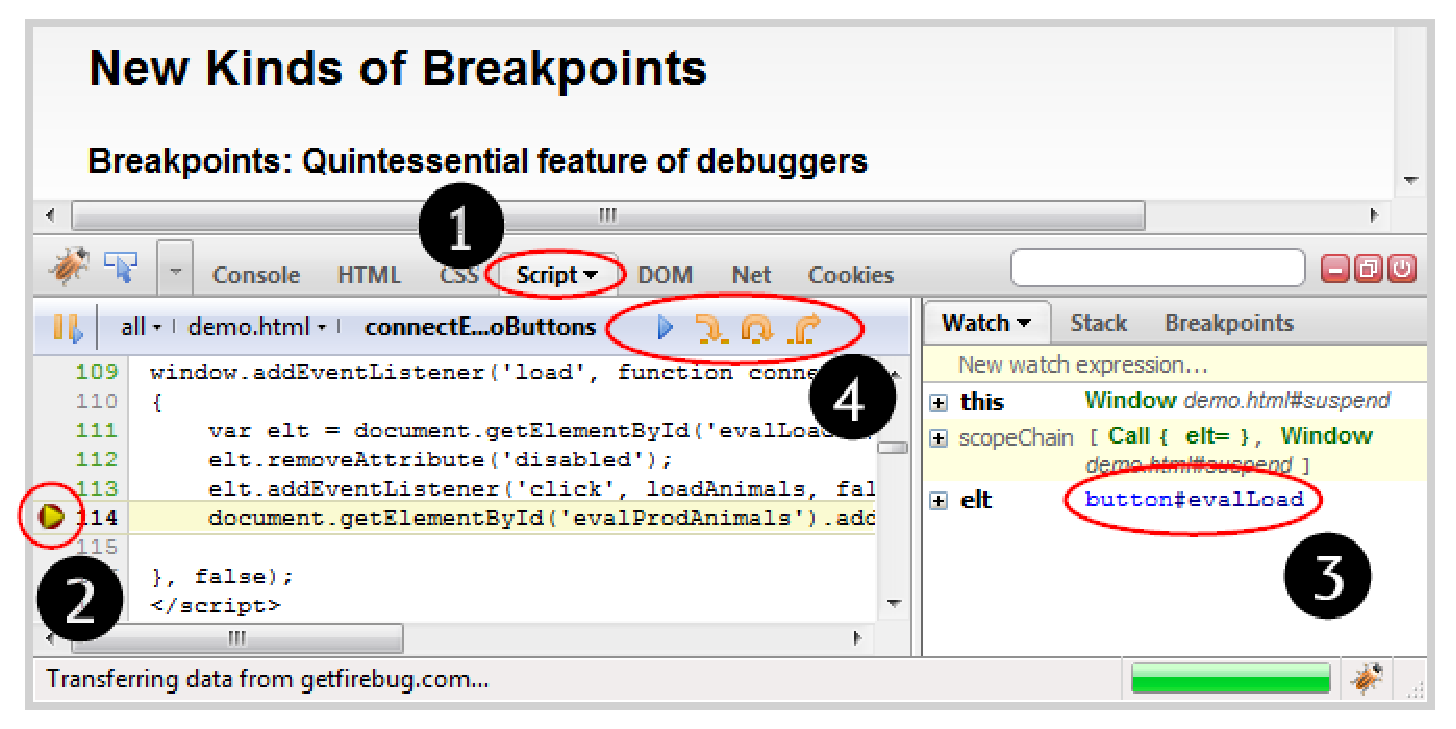
\includegraphics[scale=0.7]{FirebugOnBreakpoint.eps}
\caption{Lower part of a Web page with the Firebug debugger open. The
developer has selected the Script panel (tab labeled 1) and set a
breakpoint on line 114 (red dot under yellow triangle, labeled
2). Then they reloaded the page and hit the breakpoint. Note the file
name \texttt{demo.html} to the left and below the Script tab.  The yellow
triangle and yellow highlight signals the executing line. Variables in
the runtime are summarized to the left and values are summarized in
terms of the DOM. For example, the varible ``elt'' is summarized as an
HTML \texttt{button} with \texttt{id} of \texttt{evalLoad} (label
3). Place the mouse over the word \texttt{button} highlights the corresponding part of the Web page.
The developer studies the state then moves forward in execution
with the continue or step controls (label 4). }
\label{fig:firebug}
\end{figure*}

The debugger we extend is ``Firebug''\cite{getfirebug}.  In 2006, Joe Hewitt
combined ideas from
his previous work on DOMi, the Mozilla document object model
inspector\cite{HewittDOMi}, with a Javascript debugger to create a ``Web page
debugger''.  The Firebug user interface opens in the bottom of a Web page (see
Fig.~\ref{fig:firebug}).  It contains a toolbar on top of a set of
panels labeled Console, HTML, CSS, Script, DOM and Net.  (Other panels
can be added by extensions). Each panel renders information from
inside of the DOM for the Web page.  For example, the HTML panel shows
the elements of the DOM rendered as HTML.  This is not the source HTML
but rather the HTML after it has been transformed by Javascript in the
page.

Firebug's Javascript support included conventional
``breakpoints''.
To use a breakpoint, a developer navigates to a
representation of a source file, selects a line of source code and
clicks on the left side of the line (see Fig.~\ref{fig:firebug}). A
red dot marks the line as ``having a breakpoint''.  Then the developer
runs the program.  Whenever the Javascript runtime executes that line
of code, the debugger ``hits the breakpoint''.  It halts the execution
of the Web page Javascript and begins to execute debugger code to
support the developer in understanding the program state in the now
frozen Web application. Rather than examining memory directly, Firebug
allows you to examine the graphical state of the user interface using
the abstractions of HTML and CSS rather than only those of Javascript.
The developer has a graphically-integrated live-object view of the web
page at an execution point in their program.


\section{User Experience}

 In the
following sections we describe new breakpoints that help the developer
understand more complex Web applications.

\subsection{Breakpoints in Javascript from \texttt{eval()}}

\begin{figure*}[htp]
\center
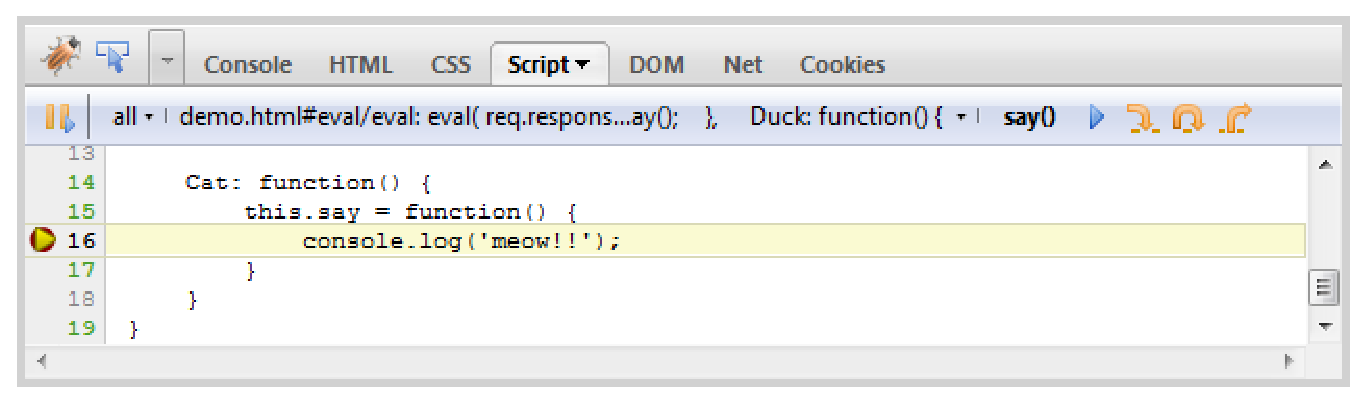
\includegraphics[scale=0.7]{script_hit_eval_md5.eps}
\center\caption{Part of the Firebug Script panel when we have set and then
hit a breakpoint in a dynamically compiled Javascript function. The
red dot appears when we click in the left gray column to show that a
breakpoint is associated with the line. Note the file name above the
source code reading ``demo.html/eval:'' followed by some of the source
code.}
\label{fig:script_hit_eval_md5}
\end{figure*}

\begin{figure*}[htp]
\center
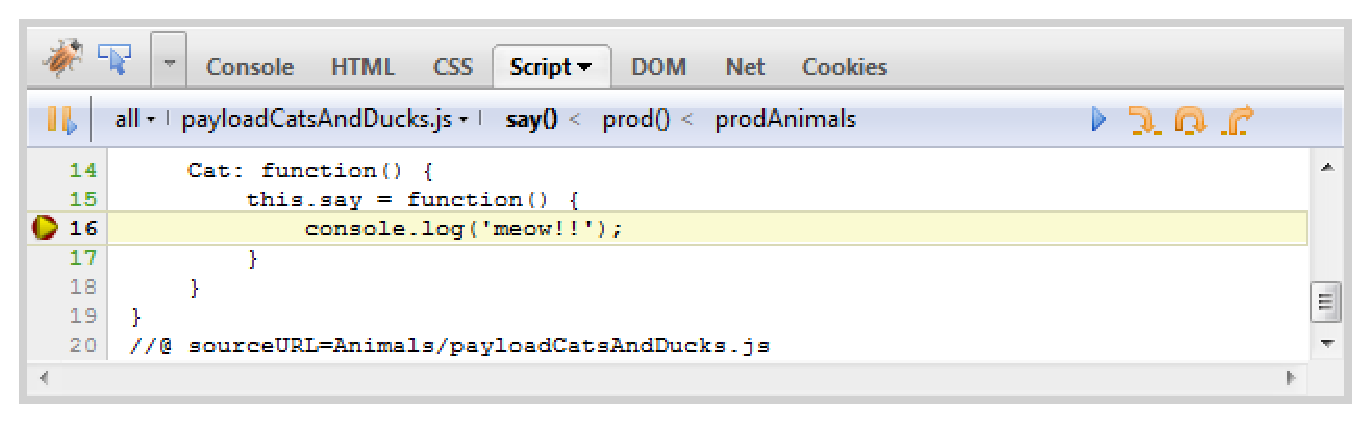
\includegraphics[scale=0.7]{script_hit_eval_userURL.eps}
\caption{As in Fig.~\ref{fig:script_hit_eval_md5}, but in this case
the developer has appended a special comment (see line 20) to specific
the name of the source. Compare the file name here to the comment and
to the file name in Fig.~\ref{fig:script_hit_eval_md5} }
\label{fig:script_hit_eval_userURL}
\end{figure*}


Javascript supports the creation of new executable functions at
runtime with the \texttt{eval()} function. The function takes a string
argument and compiles it; the functions defined in the string are
available immediately thereafter. In a common use of \texttt{eval()},
the string arrives in an XMLHttpRequest. For example, the 'dojo'
javascript framework uses \texttt{eval()} in the conditional construction of
an application\cite{felocity2007JIT}.  However, the string can be computed at runtime
in many ways and for many purposes.

Since the string argument to \texttt{eval()} may not be related to any
source file, the Javascript compiler associates no source file name to
the compiled functions. As a result, without something like the implementation
we describe in this paper, the functions from \texttt{eval()}
are not supported for debugging.

With our support, the user experience is wonderfully unsurprising.
By default, the debugger provides a stable but hidden file name and
all of the remaining debugger infrastructure and user
interface features work as for static sources (See Fig.~\ref{fig:script_hit_eval_md5}).

When \texttt{eval()} is used extensively and especially when the
string being compiled corresponds to a source file, the default of a
short fragment of source can be confusing. In these cases the
developer may append a special comment to the \texttt{eval()} argument. The comment
contains the file name after the string \texttt{sourceURL=} (see
Fig.~\ref{fig:script_hit_eval_userURL}).  This comment can be appended
at any time before the \texttt{eval()} call.  If the \texttt{eval()}
string corresponds to a file, the URL can be appended to the source
file.  When this comment is used, the entire debugging experience is as if the
source had been loaded from a \texttt{script} tag with the \texttt{src=}
attribute set to the value of the \texttt{sourceURL=} value in the
comment.

\subsection{Breakpoints on Errors}
\begin{figure*}[htp]
\center
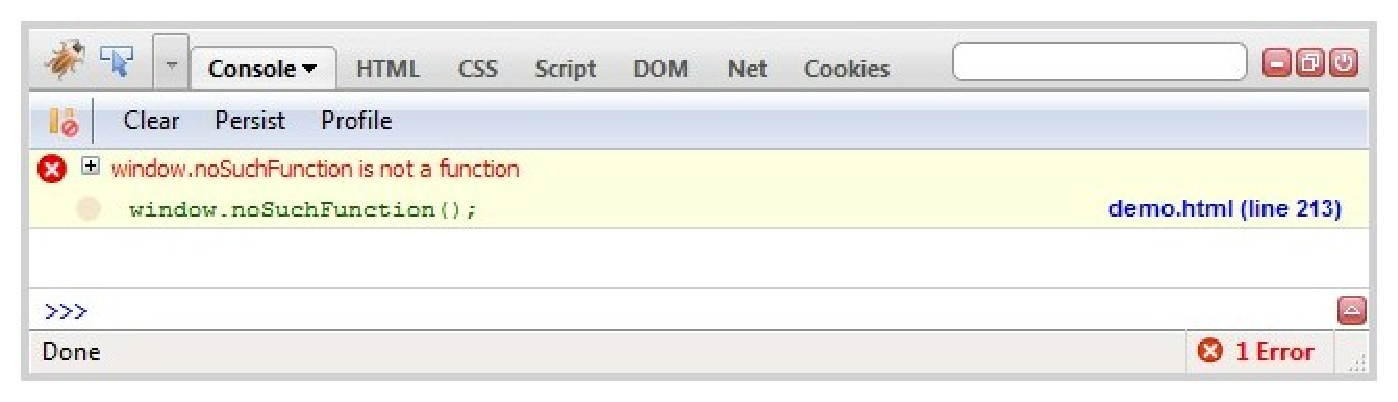
\includegraphics[scale=0.7]{error_in_console_set_break.eps}
\caption{Part of Firebug's Console panel when an error has occured in the Web
page. The small plus sign to left of the error message opens the UI to
show the call stack. Developers click on the faded red circle to set a
breakpoint on the line of the error. The circle will turn dark red.
Also note the orange parallel bars (``pause'') button used to arm the
break-on-next feature.}
\label{fig:net_set_XHR_BP.eps}
\end{figure*}
\begin{figure*}[htp]
\center
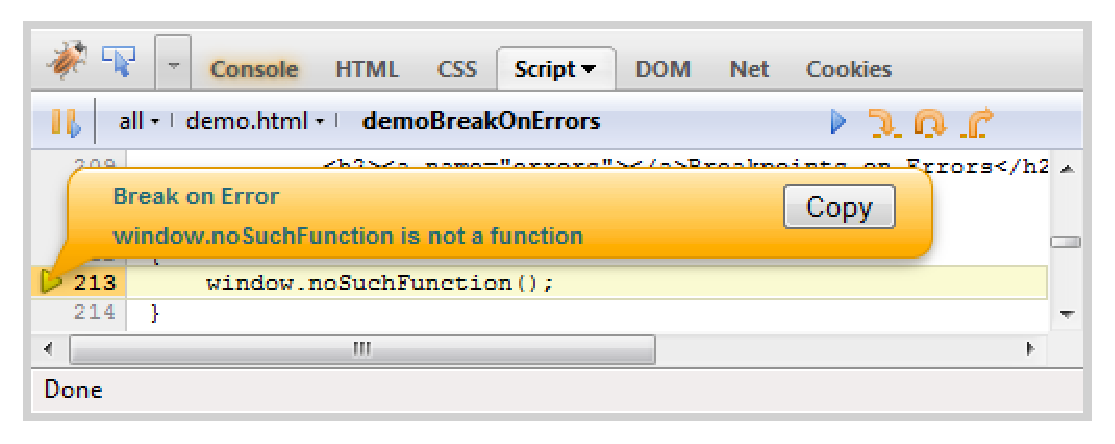
\includegraphics[scale=0.7]{console_hit_bon.eps}
\caption{Firebug's Console panel when stopped on a breakpoint after
break on next is set.  The executing line is highlighted; the error
message bubble informs the developer of the error message but also
connects the breakpoint event to the break-on-next request in the case
that multiple breakpoints may be set.}
\label{fig:console_hit_bon.eps}
\end{figure*}

In a Web browser, errors do not typically halt execution. Javascript
syntax errors abort the compile of a single file; CSS or HTML errors
abort the processing of only the containing syntax unit; uncaught
Javascript exceptions halt only the event handler that raise
them. While this gives the Web page user as good an experience as
possible given that something is wrong, developers are left without
context for errors beyond file and line information in the error
message.

Firebug offer three approaches to get more information. First, the
developer can set an option to ask that the call stack be recorded at
each error. Second,
the developer can use Firebug's Console panel to set a break point on
the source line of the error. Third, the developer can set Firebug to
break on the next error, no matter where it occurs.
We will give more detail on the second and third
cases.

When Firebug is enabled for a Web page, errors occurring in the page are
signaled to the developer with a red error counter in the browser's
status bar across the bottom. Clicking on the error count opens
Firebug on the Console panel (or selects the Console panel if Firebug
was open). The error message shows as a line along with a stack trace
to the problem and one line of source, showing where the error
occured. The developer clicks on the left end of the line to set a
breakpoint on the source code line. This is a simple form of setting
breakpoints by navigation: the developer need not know or look at the
complete source to set the breakpoint.  To trigger the breakpoint, the
page is operated again to reproduce the condition that caused the
error.

To break on the next error, the developer clicks the Console panel's ``pause''
button. This ``arms'' the feature, meaning that we don't break in to
the debugger until the next error. The
user-interface signals this change in state by changing the color
of the Console panel label
and animating the pause icon to simulate
``throbbing'' bars. When the breakpoint hits, the user interface
switches to the Script panel and the error message is shown (see
Fig.~\ref{fig:console_hit_bon.eps}).

\subsection{Breakpoints on Network Events}
\begin{figure*}[htp]
\center
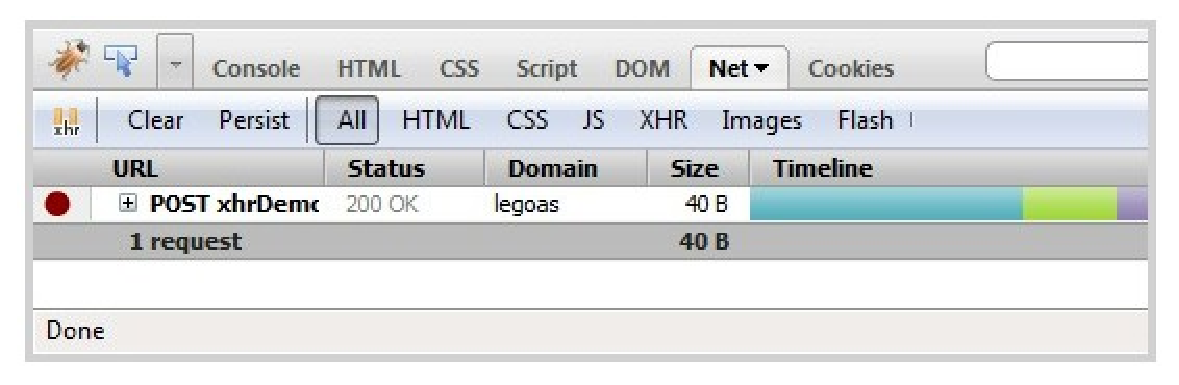
\includegraphics[scale=0.7]{net_create_breakpoint.eps}
\caption{Setting a XHR breakpoint in the Firebug Net panel view. The
developer locates the XHR request they wish to break on, and clicks in
the left column. The red dot gives the user feedback that the
breakpoint is set.}
\label{fig:net_create_breakpoint.eps}
\end{figure*}

The XMLHttpRequest introduced asynchronous data update; now
more and more web developers are using this technique to replace
traditional model where a web page is entirely reloaded every time the
user performs an action. The modern XHR approach allows loading
additional data or further parts of the application logic without
necessity to leave the current page. This dramatically improves
usability and responsiveness of a Web application.

Using dynamic XHR pattern for building online applications has
an obvious impact on amount of code that developers have to write on
the client side. The more code is involved in the network
communication,  the more effective tools for debugging are required.

Firebug already contained a tool that can be used to monitor and
analyze HTTP traffic between a client browser and the server, but
there was no integration with the Firebug debugger.  To increase
developer awareness of the breakpoint feature, we adopt a user interface
solution resembling the Script panel.  Each XHR appears on a separate
line; the XHR lines are styled with a gray cell on the left end, the
developer selects a request for breaking by clicking in the left end
(see Fig.~\ref{fig:net_create_breakpoint.eps}). This is consistent with the
source-code line display and breakpoint setting in the Script panel.

Network breakpoints halt Javascript
execution when a requests is made to a specific URL (see Fig.~\ref{fig:net_hit_XHR_BP.eps}).
To activate the breakpoint, the developer operates the Web page to cause the
XHR event.
\begin{figure*}[htp]
\center
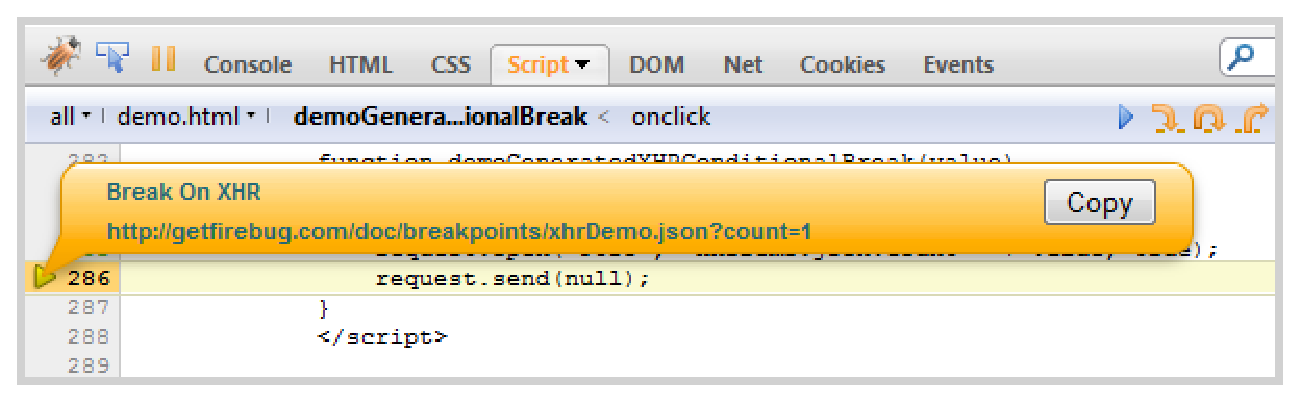
\includegraphics[scale=0.7]{net_hit_XHR_BP.eps}
\caption{Hitting a XHR breakpoint in the Firebug Script panel view. The cause of the breakpoint is given in a popup bubble over the source code line.}
\label{fig:net_hit_XHR_BP.eps}
\end{figure*}
 At the breakpoint, the usual debugging operations can
be performed and execution can be continued.


When many XHR events
occur, the developer may avoid tedious repetitive break/continue
operations by using the conditional expresssions. A right click on the
breakpoint indicator opens a one-line expression input control (See Fig.~\ref{fig:net_create_condition.eps}).
\begin{figure*}[htp]
\center
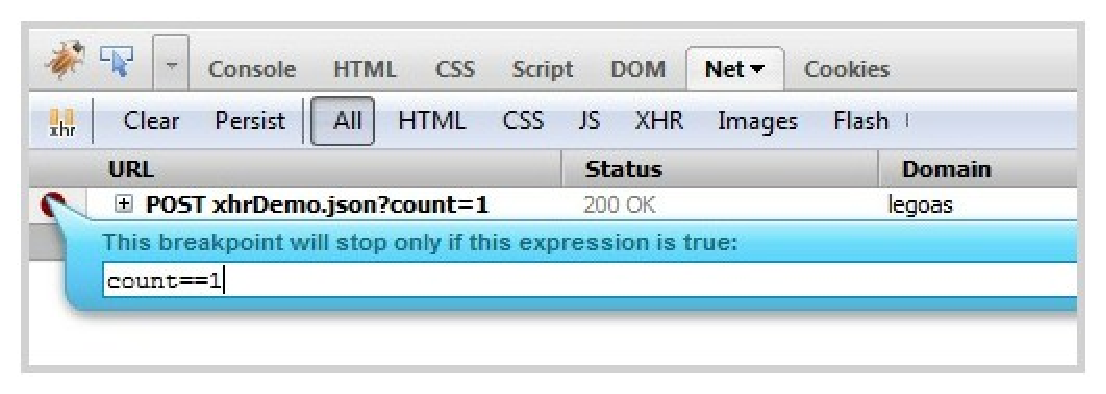
\includegraphics[scale=0.7]{net_create_condition.eps}
\caption{Breakpoint condition editor for the Net panel XHR event}
\label{fig:net_create_condition.eps}
\end{figure*}
The developer
enters an expression using URL
query string parameters or posted data. The breakpoint hits only if the expression
evaluates to true at the time of the network event.

In the opposite extreme, the developer can elect to break on the next
XHR event of any kind by clicking the yellow ``pause'' parallel bar icon
(see Fig.~\ref{fig:net_create_breakpoint.eps}).
The feature can be useful to gain understanding of the
application when the connection between XHR and Web page user
interaction is not well understood or when the XHR event timing is
unclear. This feature can be combined with the conditional XHR BP set
to \texttt{false} to skip XHR events that are understood.

\subsection{Breakpoints on HTML (DOM Mutation) Events}
\begin{figure*}[htp]
\center
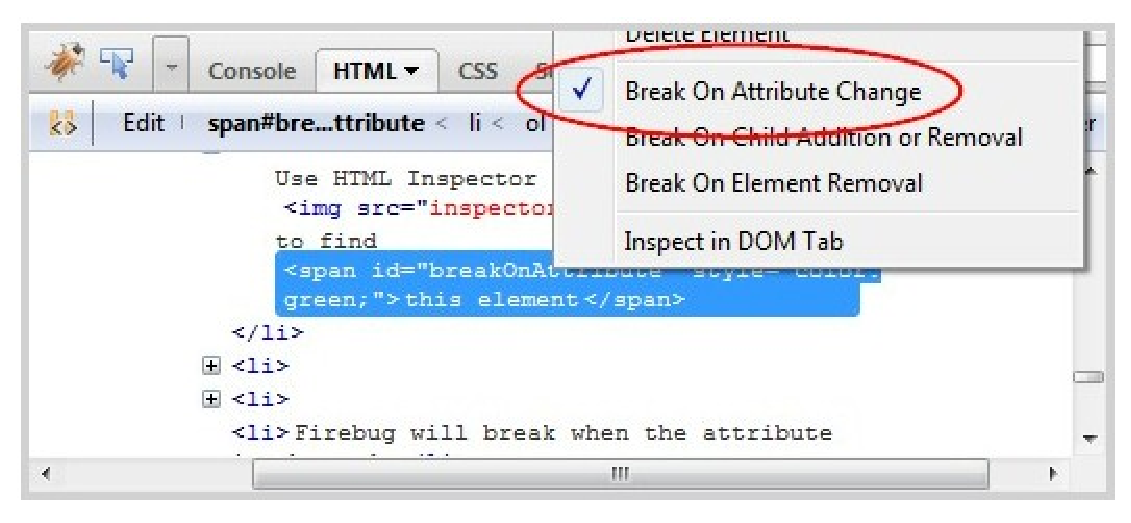
\includegraphics[scale=0.7]{html_create_breakpoint.eps}
\caption{Setting an attribute breakpoint in the Firebug HTML panel
view. The developer locates the element using Firebug's inspector 
then uses the contextual menu to set a ``break on attribute change''.}
\label{fig:html_create_breakpoint.eps}
\end{figure*}

\begin{figure*}[htp]
\center
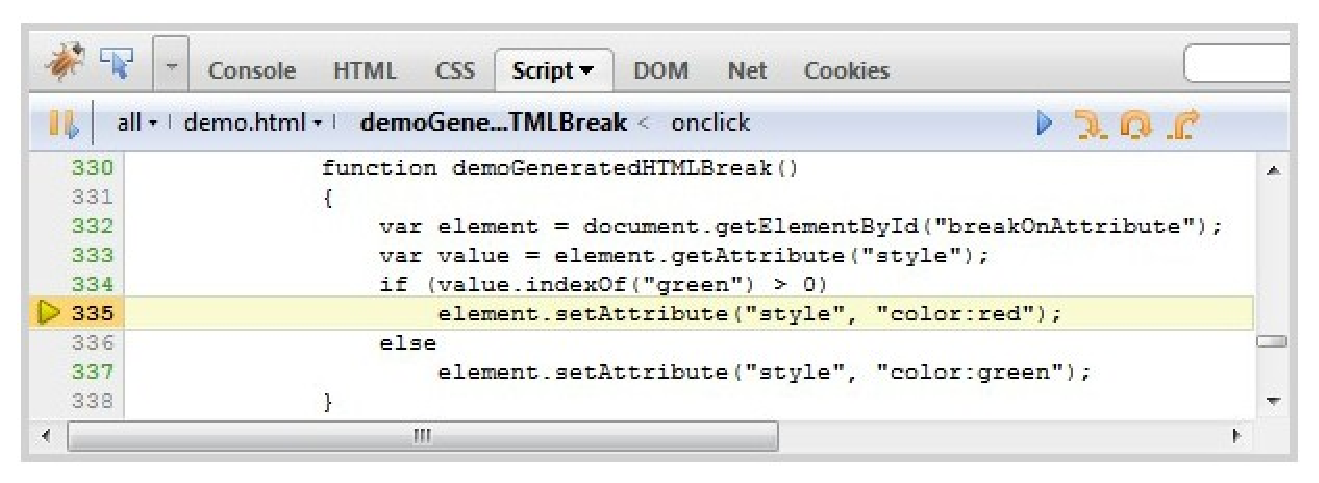
\includegraphics[scale=0.7]{html_mutation_on_break.eps}
\caption{A part of the Firebug UI when a developer has hit a breakpoint set by selecting ``Break On Attribute Change'' as shown in Fig.~\ref{fig:html_create_breakpoint.eps}. Note that this may be the first time the
developer sees the source code, all previous operations to set the breakpoint are graphical.}
\label{fig:html_mutation_on_break.eps}
\end{figure*}

Modern Web pages create dynamic user experiences in part by Javascript
UI event handlers that add or remove HTML elements or their
attributes. The programming model is not modular in graphical space or
time: any event handler can change any part of the user interface at
any time it is run. The developer then must make the connection
between changes in the UI and source code. One way to do this is to
inspect the Web page with Firebug, look through the live markup for
unique strings, then search the source code for these strings. This
activity is time consuming and distracting.


The HTML breakpoint dramatically illustrates the alternative ``recognize'' or
``browse'' approach to breakpoints. As before, a developer inspects
the Web page graphical area they want to investigate. The HTML panel
updates to show the HTML reconstruction of the current state of the
corresponding DOM element (see
Fig.~\ref{fig:html_create_breakpoint.eps}). The developer right clicks
on the element and selects one of ``break on attribute change'', child
element addition or removal, or element removal. Then they operate the
page and the debugger halts on the Javascript code that causes the
corresponding mutation (see Fig.~\ref{fig:html_mutation_on_break.eps}).
Only at this last step does the developer engage with the source code
view. The developer need not recall the source of the attribute change, but 
can arrive at the source when the breakpoint hits.


\subsection{Breakpoints on DOM Property Changes}
\begin{figure*}[htp]
\center
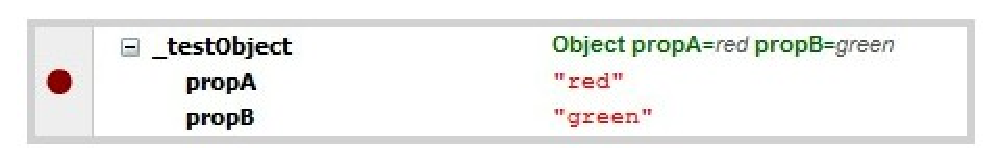
\includegraphics[scale=0.7]{dom_property_breakpoint.eps}
\caption{Part of the Firebug DOM panel, showing a breakpoint set on a property of an object.}
\label{fig:dom_property_breakpoint.eps}
\end{figure*}


A common feature of debuggers is to break the execution flow when
memory is written. In object-based languages, the debugger can express
this operation in terms of object changes.  Object properties are
shown in Firebug as name-value pairs on separate lines in the DOM (for
Document Object Model) panel. Following the style of the Net and
Script panels, the DOM panel shows a gray area on the left end of the
line. To set a breakpoint on a property change, the developer clicks
in this gray area (See
Fig.~\ref{fig:dom_property_breakpoint.eps}). When the breakpoint hits,
Firebug highlights the source lines causing the modification and
a pop-up balloon gives the old and new property values.

\subsection{Breakpoints on CSS Style Rule Changes}

As for the Net, Script, and DOM panels, the Firebug CSS panel includes a gray column to the
left of the style rules. Clicking here sets the breakpoint for changes to the corresponding
CSS rule. When the rule changes and the breakpoint hits, the script panel is selected and
the source line highlighted as in the other cases.

\subsection{Breakpoints support for Extensions}
The implementation mechanism used for most of these breakpoints is available for Firebug extensions.
This allows extensions that support higher level abstractions outside of Firebug's
core support to implement breakpoints more simply and with a consistent user interface. We
implemented breakpoints in FireCookie\cite{FireCookie2009} to ensure that the feature would work
in an extension and to give an example for other extension developers.


\section{Implementation}

Firebug works within Firefox, a production Web browser having an
underlying C++ core with a layer of interpreted graphics on
top. Firebug works entirely in the interpreted layer, using API calls
to extract information from Firefox or to manipulate the Web page.

\subsection{Dynamically Created Javascript}

To support breakpoints in dynamically created code, we need to
associate a unique identifier with the code. This identifier needs to
be robust across page reloads, since the dominant paradigm for
debugging is to set a breakpoint then reload the page to stop on the
breakpoint and examine the browser state.  For Javascript source
included with the \texttt{script} tag, the value of the \texttt{src}
attribute provides such an identifier.  Dynamic functions have no
source file as far as the browser is concerned. The compiler sees only
a string, the argument to \texttt{eval(str)}.  The string may be
prepared in memory just before execution and the developer may never
have seen the particular instance executing.

In the particular case of the Firefox browser, obtaining the string
passed to the compiler involved manipulating the javascript runtime
through the debug interface. The compiler provides notification of
compilation (\texttt{onScriptCreated}) but not source compiled nor an
indication of whether that source is from \texttt{eval()}, a
\texttt{script} tag, or a browser generated source.  To distinguish
these cases it was necessary to set a breakpoint in the compiled code
at program counter zero and, when the engine hit the breakpoint,
examine the call stack heuristically. Ideally this approach would not
be necessary, but it is worth noting that a debugger has this ability
to create such un-conventional control flows.

Given the source string we need a unique identifier for it.  Our
initial implementation followed previous suggestions to encode the
source string as a 'data:' URL\cite{Bugzilla307984}. The 'data:' URL is a valid
input to various parts of the brower, making it attractive for this
purpose and for small programs this approach was effective. However
the performance of this implementation was unacceptably slow, probably
because it more than doubles the memory required for source files and
the encoding algorithm is not highly optimized.

We reimplemented the identifier computation in two ways.  First, as 
described in Sec. 3.1, we
look for a sentinel string at the end of the \texttt{eval()} string
giving a user-defined value for the identifier; this can be used by,
for example, to connect the compiled source to the download
URL.  Second, we use the browser's builtin MD5 hash computation
function to create a 128 bit identifier very likely to be unique to
the string.  The built-in function for MD5 is highly optimized. 
The sentinal string methods works even if the developer modifies the 
source; the MD5 method works even if the developer does not or cannot 
add the sentinal string. These two combine to support the needs of most 
development use cases.

Attempts to apply the same solution to functions created by
Javascript's \texttt{new Function} feature failed because the heuristics to
access the source string became too complex. Additional support from
the browser will be needed for that case.

Firefox also generates functions, for example, to implement `click'
event handler.  These functions wrap an expression given within HTML
markup.  We support debugging these generated handlers by decompiling
their Javascript bytecodes using a service provided by the Firefox Web
browser API. We could have used this decompilation for the dynamic
code. However the decompiled code has no comments, is reformatted, and
has different line numbers from the original dynamic code. The user
experience cannot resemble debugging normal source files.


\subsection{Breakpoints on Errors}

Error-selected source-code line breakpoints simply set a conventional
source code breakpoint on the line indicated by the error
message. Thus they are a user-interface short hand.

The break-on-next exception
implementation relies on the Firefox engine's \texttt{onError()}
method, called for every exception. When \texttt{onError()} is called
we don't directly enter the debugger's user interface code. Rather we
call a method \texttt{breakNow()} which sets a break-cause object
containing the error message and then executes a single Javascript
statement \texttt{debugger;}. This triggers the JS engine to call our
\texttt{onDebugger()} handler function. In this handler we examine the
stackframes, skip frames from the debugger itself, then find the file
and line number for the developer's frame. We pick up the break cause,
position the source code view to the file and line, and pop up a
bubble giving cause of the break, an error message in this case.  The
\texttt{breakNow()} function is used for many of our breakpoints to
increase code reuse and ensure a consistency in the user experience.


\subsection{Breakpoints on Network Events}

Firebug intercepts network requests and responses to implement the Net
panel view. On each event we compare the URL to a list of breakpoints;
matches are further tested with conditional expression evaluation if
required. Successful matches set the breaking cause object to the XHR
event and call the \texttt{breakNow()} function described above.


\subsection{Breakpoints on HTML (DOM Mutation) Events}

The W3C DOM Events standard\cite{Pixley2000Events} implemented by Firefox supports DOM
mutation events raised for each change in the DOM. The breakpoint
implementation for the HTML panel simply adds listeners for each DOM
mutation event and calls the \texttt{breakNow()} function described above.

\subsection{Breakpoints on DOM Property Changes}

Firefox supports a \texttt{watch()} method available for all
objects. The method (if defined) is called whenever an object property
value is set. The breakpoint implementation simply defines the \texttt{watch()} to call
\texttt{breakNow()} as described above.

\subsection{Breakpoints on CSS Style Rule Changes}

No standard nor Firefox specific API supports notification of CSS
changes. We implemented CSS breakpoints by inserting a shim API layer in
the web page for every CSS-changing API call. For example, we define a
new function for
\texttt{CSSStyleDeclaration}.\texttt{prototype}.\texttt{setProperty()}
that checks if this property has a breakpoint set. If so, the breaking
cause is set to CSS property change and the \texttt{breakNow()}
function is called. Whether or not we enter the breakpoint, we call
the original function to complete the developer's intent.

A major complicating factor for this implementation is the
requirements of Web browser security.  The shim functions must be
compiled into the Web page, but we cannot call \texttt{breakNow()}
directly from the Web page. Therefore we must request
\texttt{breakNow()} by raising an event on an element in the Web
page. In Firebug, a listener for these events makes the actual function
call. Because of this extra complexity, we did not deploy the CSS breakpoints 
in production versions of Firebug.  We are currently working with the 
Firefox team to find a better alternative.

\section{Discussion}

We added support for dynamic Javascript to Firebug in 2007.
Based on bug reports, blog and newsgroup postings, the feature
is effective and used. The ``break on errors'' feature has also been a part of
recent version of Firebug, with a different user interface control.
Feedback from the ``break on next error'' feature
indicated that it was both useful for many users,
but also triggered too often for other users. Discussion of these problems
led us to generalize the breakpoints as we report here.

The remaining breakpoints are only now available in Firebug. We do not as yet have
objective evidence that these approaches are effective.
We chose not to invest in an isolated user study of these features.
As developers ourselves, we believe that the concept behind these breakpoints are
compelling and a small scale user study would not add significant new information.
To be correct, a user study requires developers to be skilled in the
use of the breakpoints and yet it would require developers
unfamiliar with the breakpoints as control subjects. These requirements conflict and they make any
such study very time comsuming.

On the other hand, since Firebug is widely used, we have an attractive alternative:
measure adoption of the breakpoints. We anticipate being able to report on the adoption
of these features early in 2010.

We chose Firebug as the base for our work on breakpoints for five
reasons: 1) when we started our work it was the only Web debugger
(other Javascript-only debuggers were available but they would have
required much more work), 2) both Firebug's entire source code and the
source for Firefox's debugging support code are readily available, 3)
Firebug is implemented in Javascript, a well-supported and
garbage-collected language easing development, 4) Firebug's open BSD
source code license allows unemcumbered commercial redistribution
helping us to support our work, 5) Firebug has an active developer and
user community providing a ready source of feedback. After we started
this work, web debuggers appeared for Opera (DragonFly) and Internet
Explorer 8. (Web Inspector for Safari has features similar to parts of
Firebug but no support for Javascript debugging). We believe that all 
of the techniques we describe here could be implemented in any of 
these other Web debuggers.

\section{Related Work}

Existing debuggers, for example Eclipse, support source code
breakpoints and breaking on exceptions.  Eclipse's break on exception
supports breaking based on the type of the error object, while our
break on next error has no such filter. The Java types are known in
advance because of Java's static typing, but of course the type of the
actual error is not known until runtime.  Once the error occurs, we
support setting a breakpoint directly on the source line.

ZStep\cite{Lieberman95bridgingthe} supports integration of graphical
objects and source code. Our approach is quite different since the Web
page run time model allows any Javascript function to operate on any
part of the page. This means that the binding of an object and the
source is only meaningful during the function invocation. For that
reason our integration uses breakpoints and re-running the code to
find the connection.

As a specialized debugger, Firebug resembles debuggers for
domain-specific languages\cite{Wu04DomainEclipse}. However, the
breakpoints we introduce here support higher-level graphical and
network abstractions, not higher-level source-code
abstractions. Firebug has domain-specific breakpoints but when they
hit, you are in general purpose source code.  On the other hand, the
extensive integration of Javascript and HTML/CSS in the Document
Object Model combined with Firebug's integration of debugger views and
the Web page blurs the line. 

WhyLine\cite{Ko2008WhyLine} supports integration of graphical state and source code
though queries into data created while running a program. The queries
are generated by demonstration on the graphical user interface. When
successful, this approach can lead directly to the source that caused
the transition demonstrated. In our approach, multiple breakpoints
might be hit before you find the one place in the source that
causes the graphical change of interest; we mitigate this problem with
conditional breakpoints. Our breakpoints have much less run time
overhead and build on existing developer experience.

FireCrystal\cite{Oney2009Firecrystal} records Web page and sequences
of diffs to support a graphical time line view of the page. Sweeping
along the time line can be used to navigate to a graphical transition
visually. The transitions are connected to the code running at that
point in the time line. Our approach is more ``spatial'' and causes
minimal run time overhead, but broadly they should be quite
complementary.

\section{Future Work and Conclusion}
The breakpoints we have introduced here fit easily into the Firebug
user interface and, consequently, the UI operations needed to set them
are easy to explain to developers.  There are cases where more complex
solutions may be needed.
For example, developers need to know why
an element has the color ``green'' independent of whether that color came
from CSS parsing, changes to element attributes (for example CSS
\texttt{class} or \texttt{style}), changes to the structure of the
document that caused new CSS rules to apply, or changes to the CSS
rules themselves.

Firebug provides good tools to master ``space'', both the 2D space of
the Web page and the interface to the network. Our breakpoints help
connect these spatial dimensions to the source code that modifies
them. But breakpoints are intrinsically ``at the wrong time'':
developers set them then run the program to hit them at a later
time. This limits the kind of immediacy of debugging advocated by
Ungar et al.\cite{Unger97Immediacy}.

Omniscient Debugging\cite{Lewis2003Omniscient}, WhyLine\cite{Ko2008WhyLine}, and
FireCrystal\cite{Oney2009Firecrystal} point to powerful new approaches to temporal
issues in debugging.  Omniscient Debugging records information while a
program runs to support reversal of control flow, that is working
backward in time.  Recent improvements reduce the overhead of
Omniscient Debugging from 100 times to more like 7
times\cite{Lienhard08OOBack}.  Since Javascript
event-handlers often complete in less than a second, real-time
recording may be feasible even in Javascript and we still have the
potential for more performance by implementing the recorder in the
C++.

WhyLine requires similar recording but adds queries as a navigation
solution. Finding ways to introduce Web developers to query based
debugging would be an important step towards realizing the potential
of these new techniques.

FireCrystal demonstrates some of the potential of trace recording
integrated with graphical recording to address the ``why is this
green'' question.  Since it is implemented in Javascript, it provides
a direct prototype for exploring the integration of trace based
solution with breakpoint based solutions and for exploring how the
developer community can become successful with the tracing solutions.

Debugging is a special challenge in highly dynamic graphical Web pages.
We think our breakpoints are in important improvement and a first step towards
providing much better support for developers. There are many more steps needed
and we hope this paper will encourage others to see that new debugging tools are
feasible and exciting to create.


%ACKNOWLEDGMENTS are optional
\section{Acknowledgments}
The Firebug project is an open source project and we gratefully
acknowledge inputs from many users and developers that shapes our
thinking on these paper. We thank Prof. Eric Tanter, Prof. Brad Myers,
Tessa Lau, Salman Mirghasemi, and Jeff Nichols, for timely and
valuable suggestions on the paper.


\begin{thebibliography}{10}

\bibitem{breakpointsDemoPage}
J.~J. Barton and J.~Odvarko.
\newblock Firebug breakpoints demo, 2009.
\newblock \url{http://getfirebug.com/doc/breakpoints/demo.html}.

\bibitem{felocity2007JIT}
J.~Heuser.
\newblock Just in time loader for javascript, 2007.
\newblock
  \url{http://www.felocity.org/blog/article/just_in_time_loader_for_javascript%
/}.

\bibitem{getfirebug}
J.~Hewitt.
\newblock Firebug: Web development evolved, 2007.
\newblock \url{http://getfirebug.com}.

\bibitem{HewittDOMi}
J.~Hewitt.
\newblock {\em DOM Inspector}, 2009.
\newblock \url{http://en.wikipedia.org/wiki/DOM_Inspector}.

\bibitem{Ko2008WhyLine}
A.~J. Ko and B.~A. Myers.
\newblock Debugging reinvented: asking and answering why and why not questions
  about program behavior.
\newblock In {\em ICSE '08: Proceedings of the 30th international conference on
  Software engineering}, pages 301--310, New York, NY, USA, 2008. ACM.

\bibitem{Ko06anexploratory}
A.~J. Ko, B.~A. Myers, S.~Member, M.~J. Coblenz, and H.~H. Aung.
\newblock An exploratory study of how developers seek, relate, and collect
  relevant information during software maintenance tasks.
\newblock {\em IEEE Transactions on Software Engineering}, 32:971--987, 2006.

\bibitem{Lewis2003Omniscient}
B.~Lewis.
\newblock Debugging backwards in time.
\newblock In {\em Fifth International Workshop on Automated Debugging (AADEBUG
  2003)}, 2003.
\newblock \url{http://xxx.lanl.gov/abs/cs.SE/0309027/}.

\bibitem{Lieberman95bridgingthe}
H.~Lieberman and C.~Fry.
\newblock Bridging the gulf between code and behavior in programming.
\newblock In {\em CHI'95: Human Factors in Computing Systems}, pages 480--486.
  ACM Press, 1995.

\bibitem{Lienhard08OOBack}
A.~Lienhard, T.~G\^{\i}rba, and O.~Nierstrasz.
\newblock Practical object-oriented back-in-time debugging.
\newblock In {\em ECOOP '08: Proceedings of the 22nd European conference on
  Object-Oriented Programming}, pages 592--615, Berlin, Heidelberg, 2008.
  Springer-Verlag.

\bibitem{FireCookie2009}
J.~Odvarko.
\newblock Firecookie, 2009.
\newblock \url{http://www.softwareishard.com/blog/firecookie/}.

\bibitem{Oney2009Firecrystal}
S.~Oney and B.~Myers.
\newblock Firecrystal: Understanding interactive behaviors in dynamic web
  pages.
\newblock In {\em IEEE Symposium on Visual Languages and Human-Centric
  Computing}, 2009.

\bibitem{Pixley2000Events}
T.~Pixley.
\newblock Document object model (dom) level 2 events specification, 2000.
\newblock \url{http://www.w3.org/TR/DOM-Level-2-Events/}.

\bibitem{Bugzilla307984}
J.~Ross and B.~Eich.
\newblock Bug 307984 - line numbers in errors from evalinsandbox are incorrect,
  2005.
\newblock \url{https://bugzilla.mozilla.org/show_bug.cgi?id=307984}.

\bibitem{Singer97anexamination}
J.~Singer, T.~Lethbridge, N.~Vinson, and N.~Anquetil.
\newblock An examination of software engineering work practices, 1997.

\bibitem{Unger97Immediacy}
D.~Ungar, H.~Lieberman, and C.~Fry.
\newblock Debugging and the experience of immediacy.
\newblock {\em Commun. ACM}, 40(4):38--43, 1997.

\bibitem{Wu04DomainEclipse}
H.~Wu, J.~Gray, and M.~Mernik.
\newblock Debugging domain-specific languages in eclipse, 2004.

\end{thebibliography}


\end{document}
